%SUBSECTION - control
\subsubsection{Simulation results}

In order to predict the behavior of the car to a linear speed reference and angle of tilt (teta), some simulations were necessary. The output of the simulation is the plot of the linear speed of the car, the linear speed of both wheels (left and right) and the position of the car.
In order to plot the position of the car the Cartesian referential is used.\\
As the controller in use is a discrete PID, the first step is to find the optimal parameters.
For the first set of simulations, the aim is to find the values for the PID gains. As purpose of the car is to explore hazardous areas, the parameter Kd will be set as 0 due to the noise. 
For the first simulation, Kd=1, ki=1, Linear speed= 1m/s, teta=0rad:
\begin{figure}[!h]
\centering
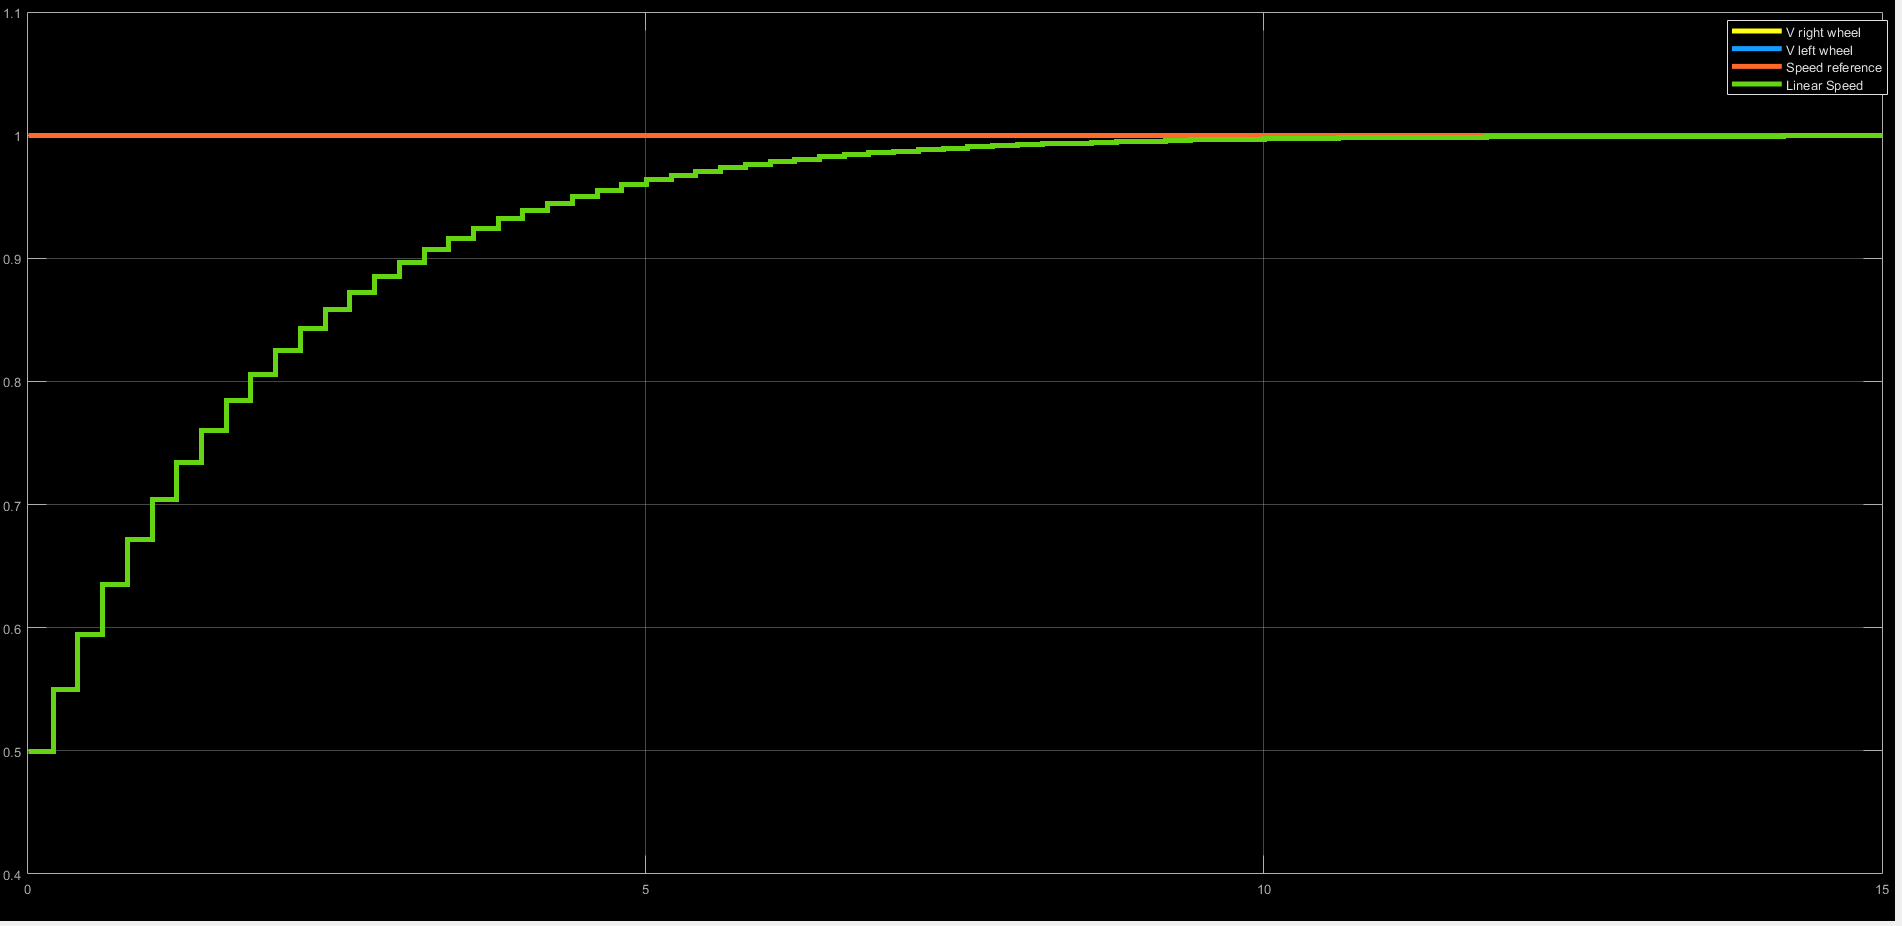
\includegraphics[width=1.0\textwidth]{./img/pid11.png}
\caption {\label{fig:pid1 - p1i1}Kd=1, Ki=1}
\end{figure}
With this simulation, it is possible to see that the initial value of the velocity of the car is 0.5 m/s and it take about 7 seconds to reach steady state. 0.5m/s as an initial value for the linear velocity is a considerably high value and can cause the car to slide, therefore, the Kd value needs to get lower, for the initial value to get lower as well.
\newpage
In this simulation, Kd will be set as 0.5 and Ki as 1.
\begin{figure}[!h]
\centering
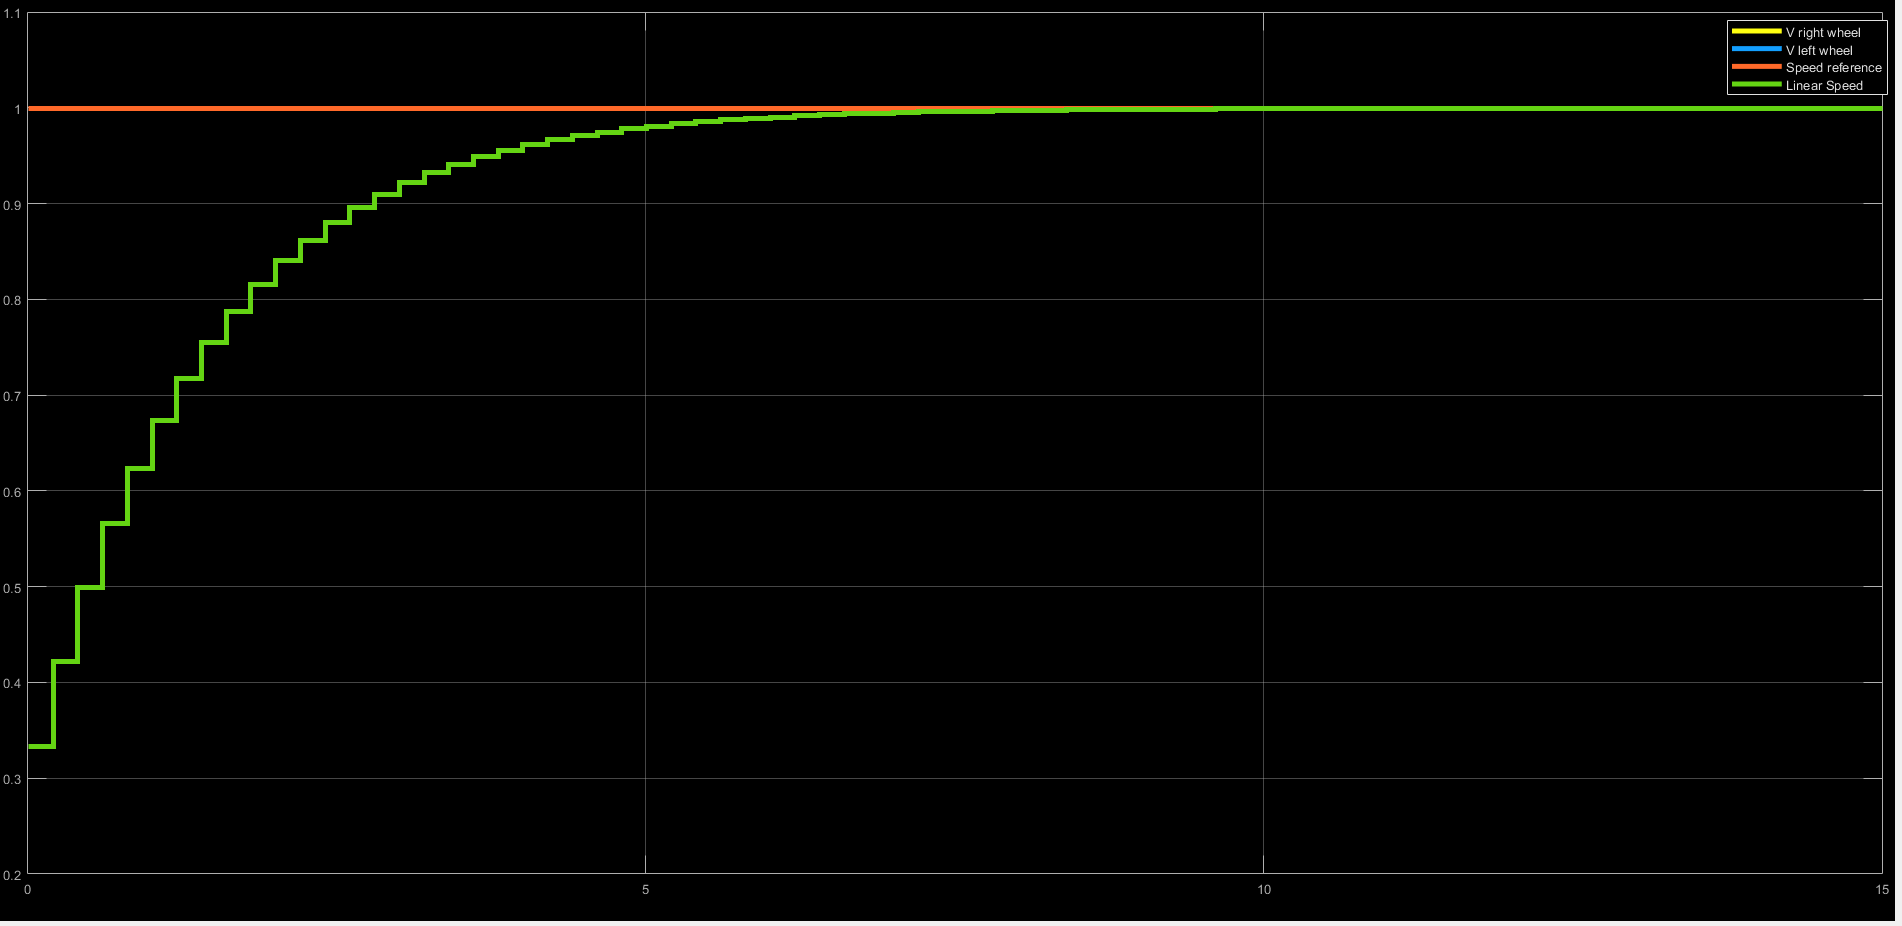
\includegraphics[width=1.0\textwidth]{./img/pid051.png}
\caption {\label{fig:pid1 - p05i1}Kd=0.5, Ki=1}
\end{figure}
Changing the value of Kd to half of the initial value, it is possible to see that the initial linear speed is now 0.3 m/s, making it harder for the car to slide. It takes nearly 6 seconds for the car to reach steady state, thus the Ki value must be increased.
\newpage
In this simulation, Kd will be set as 0.5 and Ki as 2.
\begin{figure}[!h]
\centering
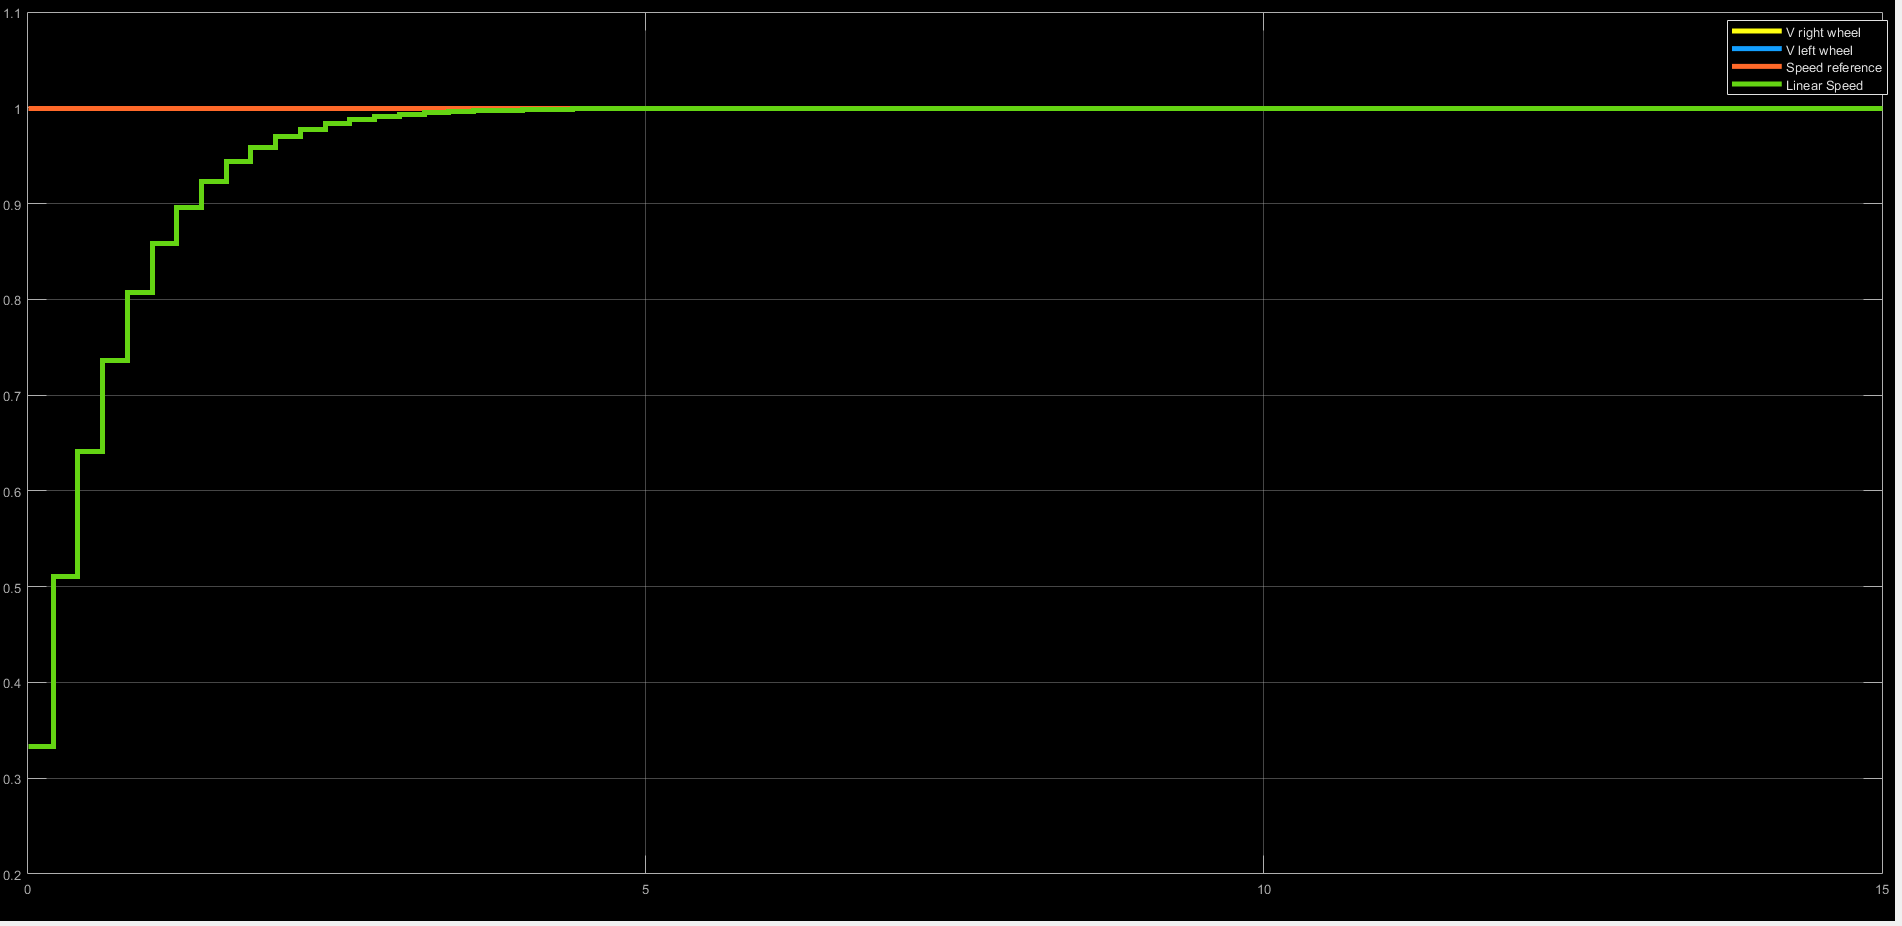
\includegraphics[width=1.0\textwidth]{./img/pid052.png}
\caption {\label{fig:pid1 - p05i2}Kd=0.5, Ki=2}
\end{figure}
As the Kd value was not changed, the initial linear speed value remains the same. As for the time it takes the car to reach steady state, it was reduced to 3 seconds due to the increase of the Ki parameter.\\
In ideal conditions, the aim would be for the car to reach the desired speed instantly, but due to the real limitations, such as wheel sliding, 3 seconds is a a safe value.
\newline
In order to choose the sample time, one needs to take in consideration that with the decrease of the sample time, the processing overhead will increase and with the increase of the sample time, the system response will have abrupt changes affecting the performance of the car. So, in order to accommodate both necessities, the sample time will be set to 50ms.
\newpage
Having determined the parameters of the controller, the next step is to simulate the response of the system.
For the first simulation, the parameters were: Speed reference= 1m/s and teta=0 rad.\\
\begin{figure}[!h]
\centering
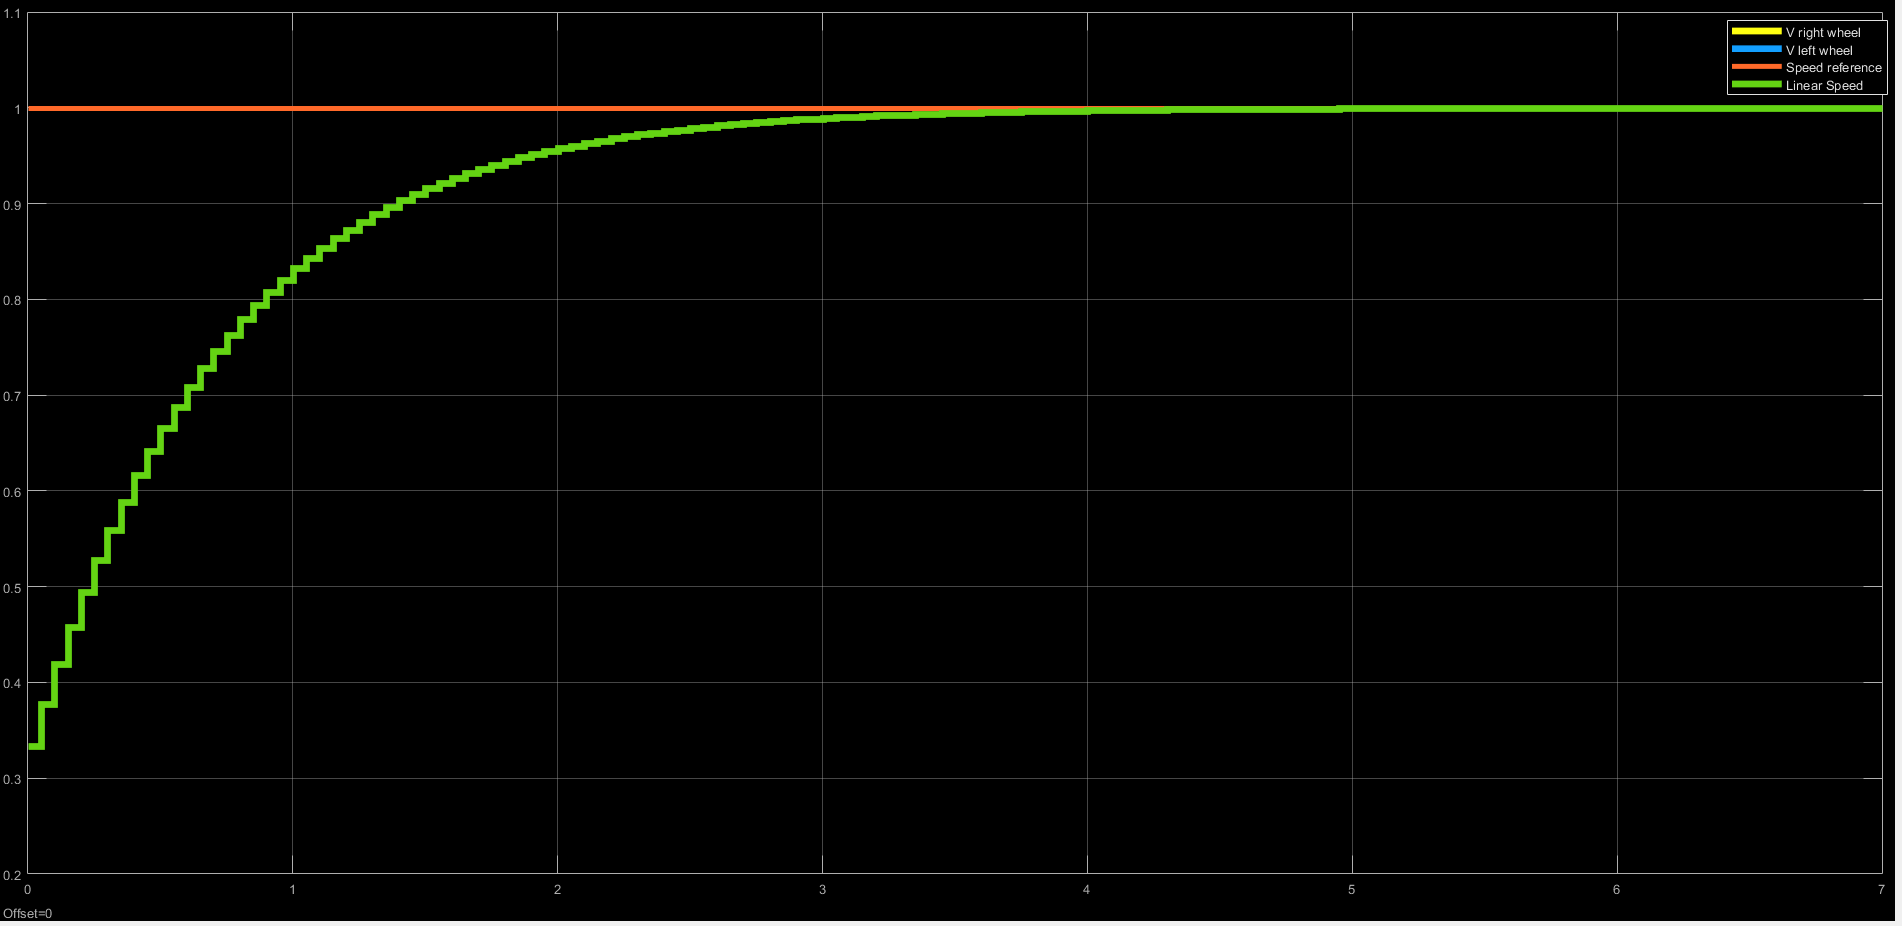
\includegraphics[width=1.0\textwidth]{./img/vel10.png}
\caption {\label{fig:sim1 - vel}Linear speed v=1m/s, teta=0rad}
\end{figure}
 As expected, the car linear velocity reached 1m/s. The angle of tilt is equal to 0 which means the car will be moving in a straight line, and as such, both wheels will are moving at the same speed of the car.\\
\newpage
\begin{figure}[!h]
\centering
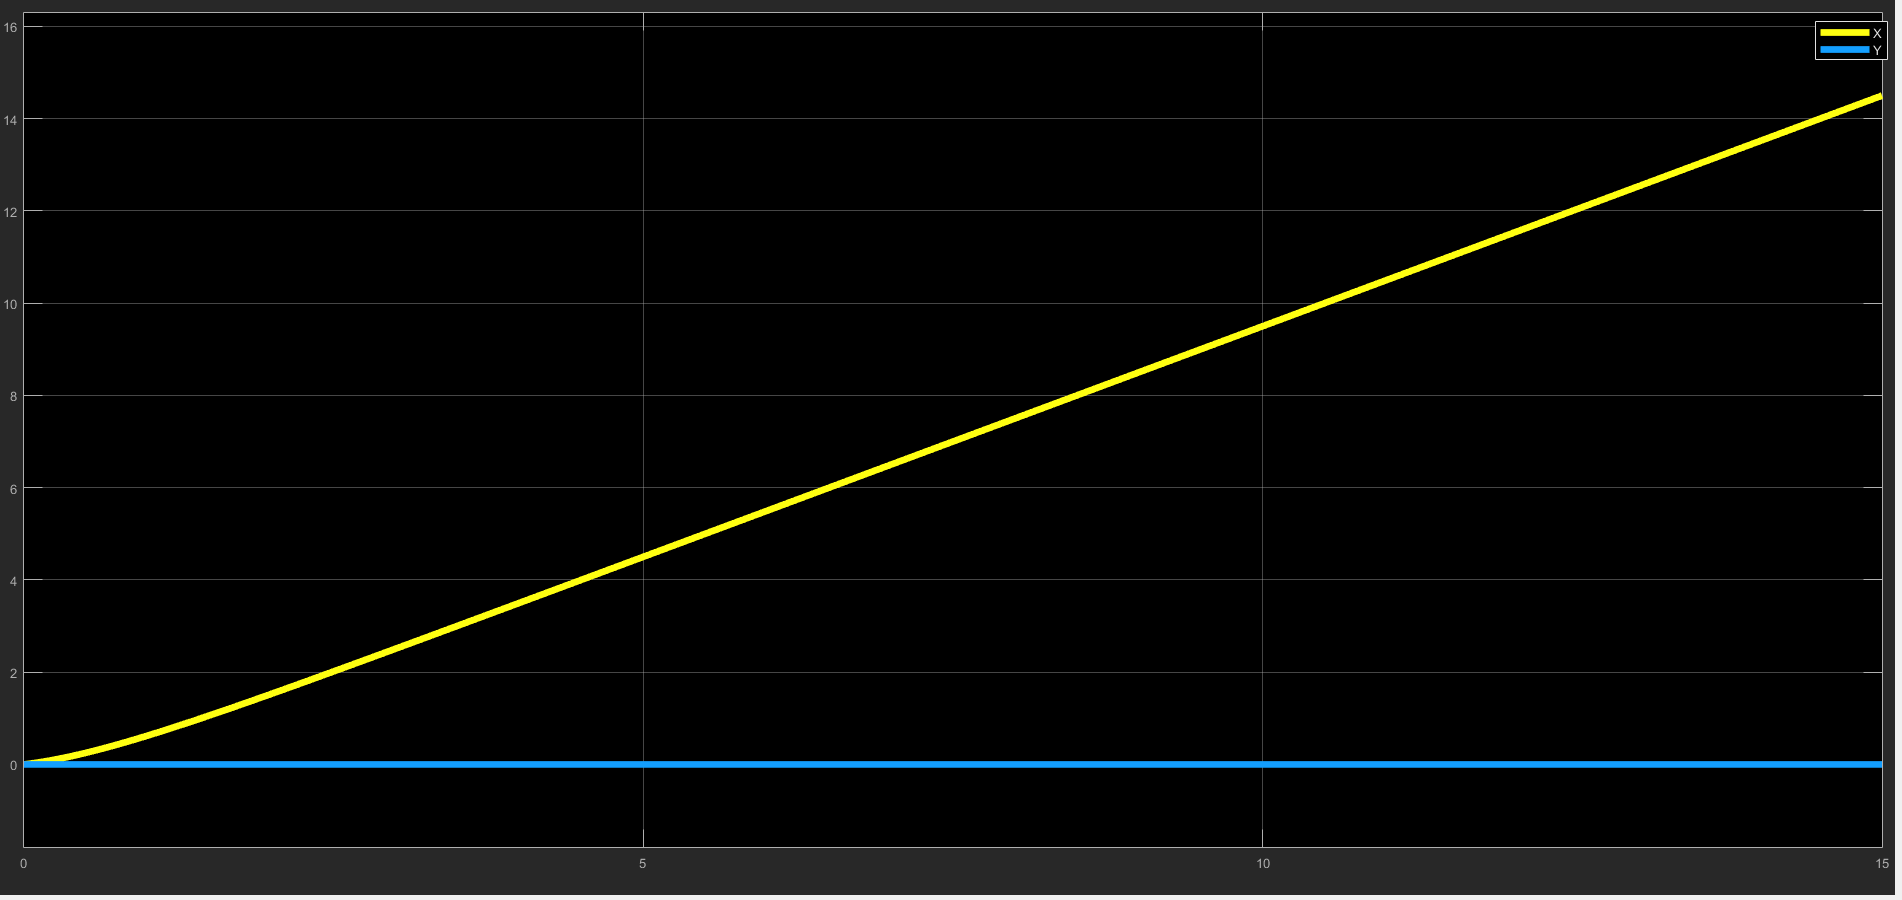
\includegraphics[width=1.0\textwidth]{./img/xy10.png}
\caption {\label{fig:sim1 - pos}Car position v=1m/s, teta=0rad}
\end{figure}
As the teta is equal to 0 rad, only 1 coordinate of the car is moving, as the figure \ref{fig:sim1 - pos} demonstrates. The x coordinate is equal to 0 the entire simulation time, and the y coordinate is increasing with a linear scope equal to the linear velocity of the car. This implies that the car is indeed moving in a straight line.\\
\newpage
Changing the teta to 0.1 rad to simulate constant tilt of the smart phone to the right, and maintaining the value of the speed reference in 1 m/s :\
\begin{figure}[!h]
\centering
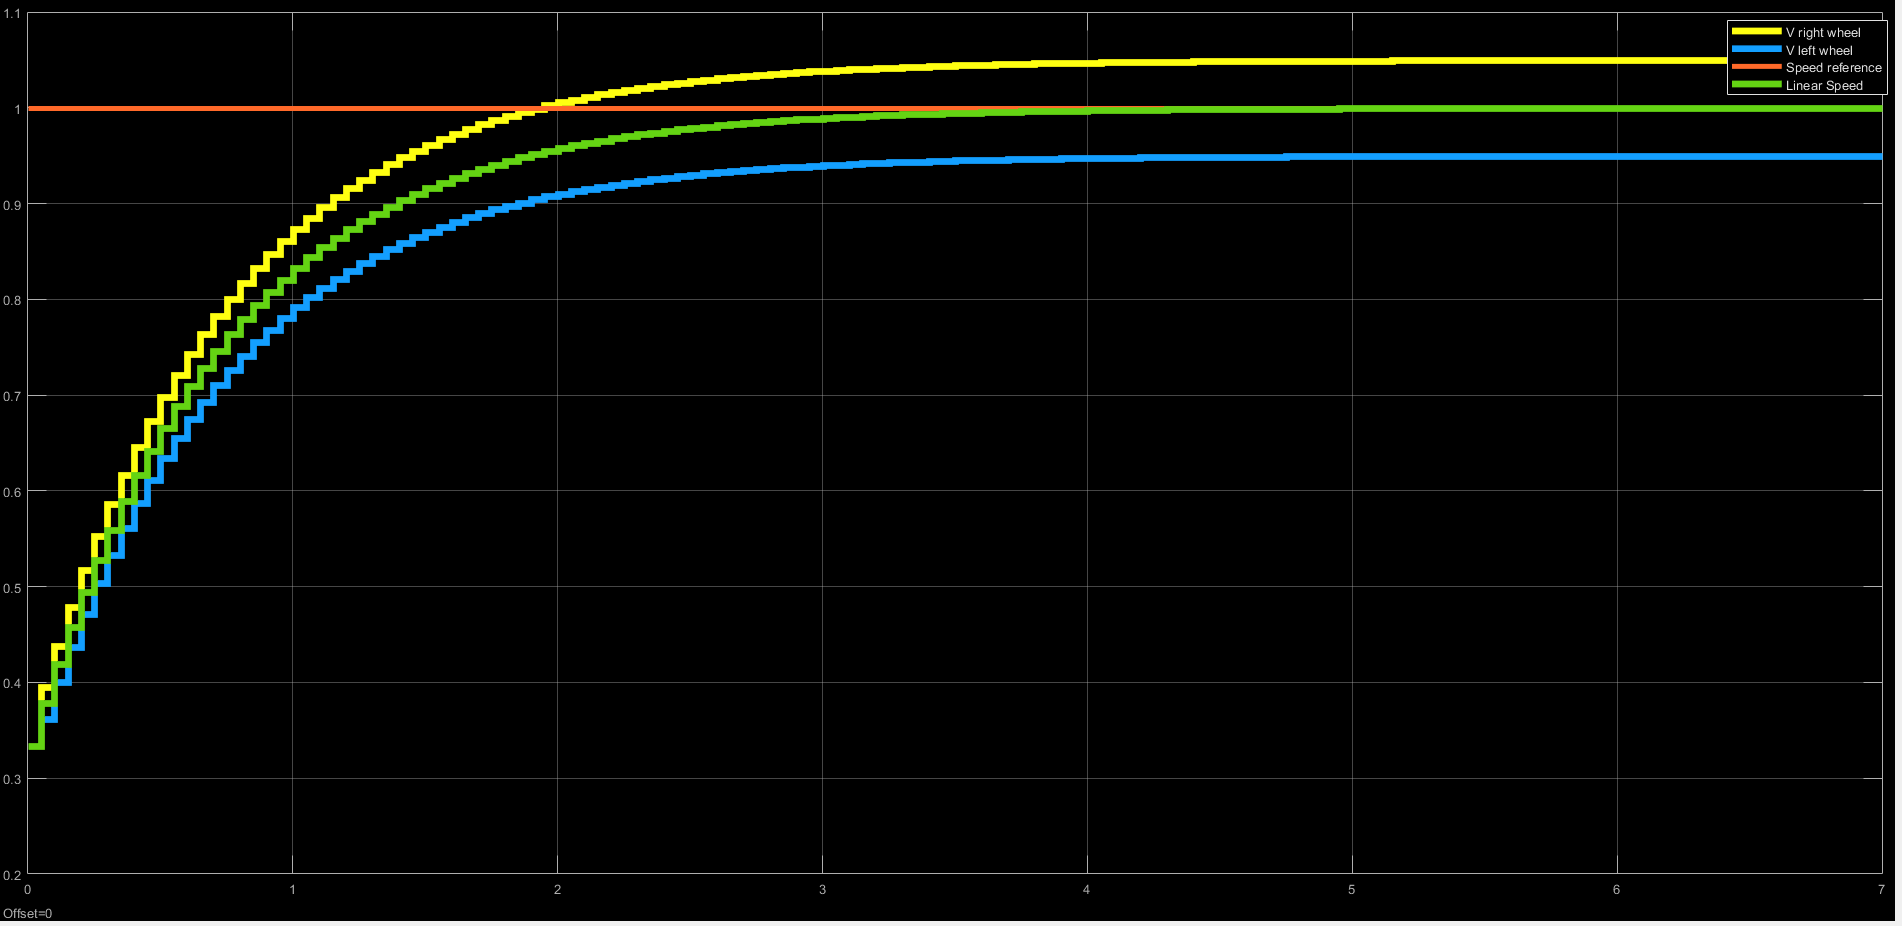
\includegraphics[width=1.0\textwidth]{./img/vel101.png}
\caption {\label{fig:sim2 - vel}Linear speed v=1m/s, teta=0.1rad}
\end{figure}
In this simulation it can be observed that having a angle of tilt not equal to 0, causes the left and right wheels to have different velocities, in order to make the car turn. Running more simulations with different values of teta, the outcome shows that the bigger the module of the value of teta, the bigger the difference between the linear velocities of the wheels.
\begin{figure}[!ht]
\centering
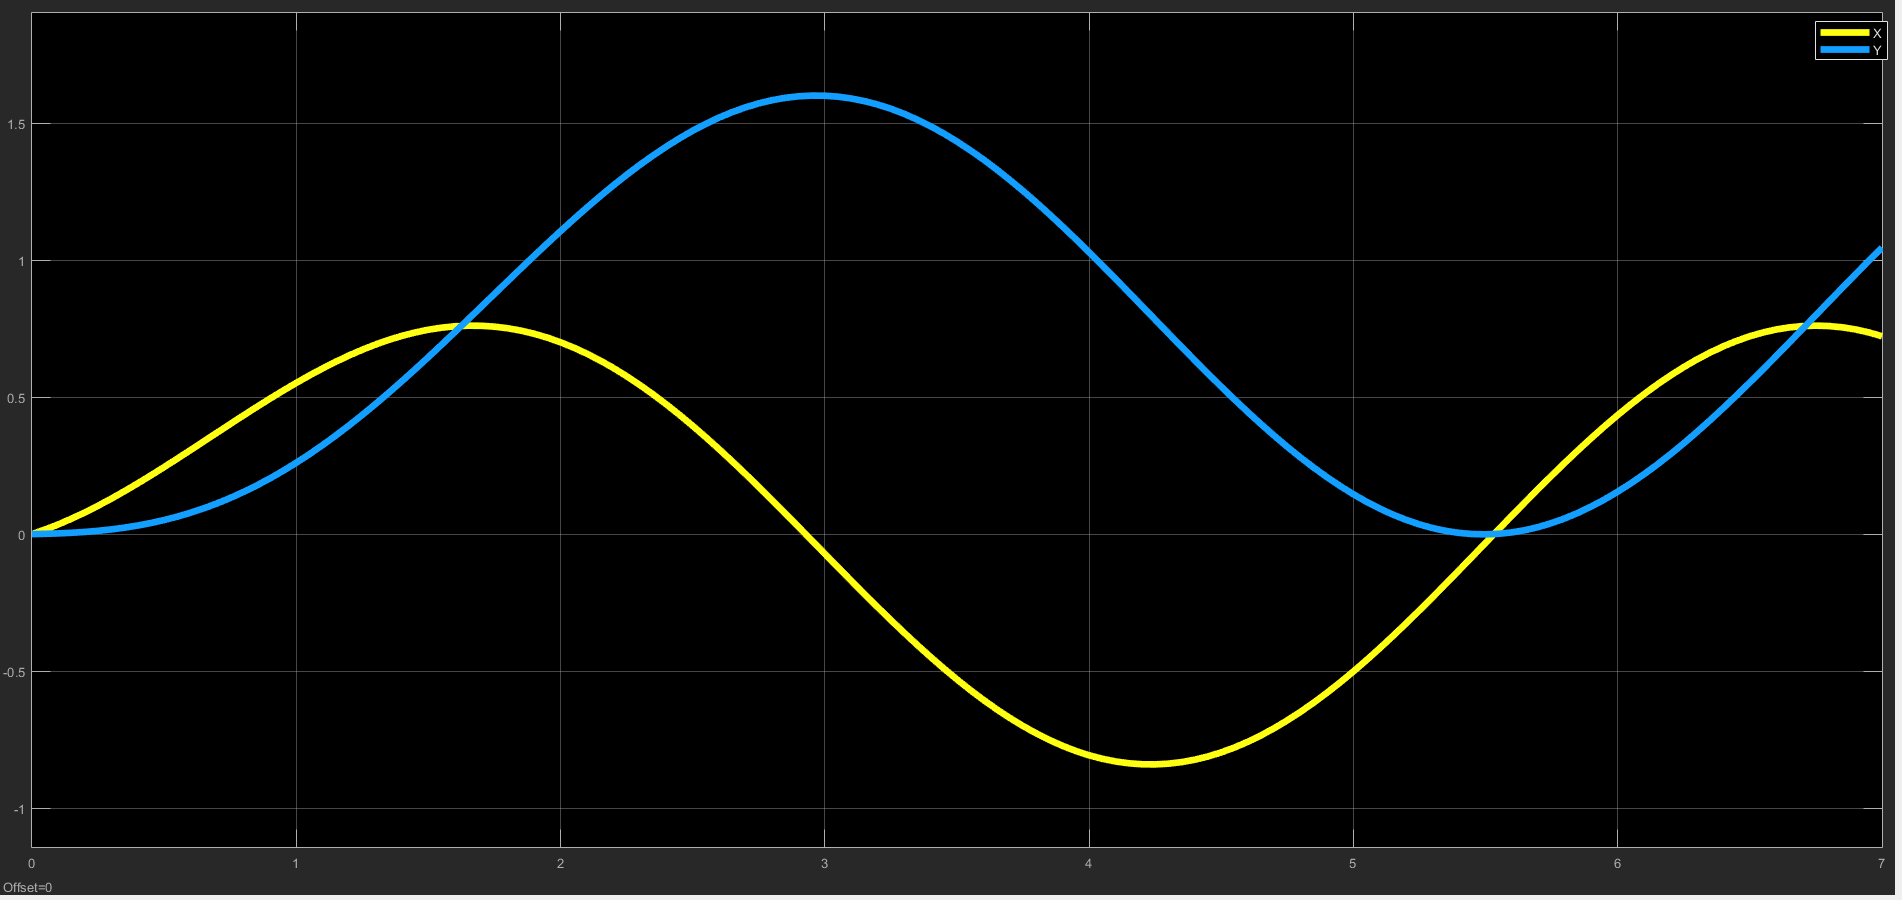
\includegraphics[width=1.0\textwidth]{./img/xy101.png}
\caption {\label{fig:sim2 - pos}Linear speed v=1m/s, teta=0.1rad}
\end{figure}
With this figure \ref{fig:sim2 - pos} it is possible to observe that both the position of x and y of the car change with time. With a constant angle of tilt, the car will turn constantly in the same direction, eventually making a 360 degrees turn and as the car as small dimensions, it takes a very small time for it to do so, which is what is observed is this simulation.